
In this chapter, we evaluate our quantification model and inference algorithms on simulated datasets with constant expected degradation rates and real direct RNA-seq datasets with sequencing spike-ins. 

\section{Read alignment}

Simulated and real reads were aligned with minimap2 \cite{Minimap2018, Minimap2021}, a popular aligner for long reads. For alignment to the genome, we used the flags \texttt{-ax splice -uf -k14} that take into account splicing and forward strand alignment for ONT direct RNA-seq as recommended by minimap2 developers. For alignment to the transcriptome, we use default flags \texttt{-ax map-ont -N10} for mapping ONT reads, keeping 10 secondary alignments due to similarities in transcript isoform sequences. We used the same genomic or transcriptomic alignments across the tools, depending on which is required as input.   

\section{Model variations}

We compare two variations of our model based on the read length-isoform agreement:

\paragraph{Deg. EM (exact)} We ran our model with the exact read length-isoform agreement model (Eqn. \ref{eq:read-iso-agreement}) and provided the known degradation rate to the model for inference. This is of course unrealistic, since in real data, the degradation rate is not known prior and there is no bound on the maximum read length (i.e., the degradation rate is not constant). Nevertheless, this serves as a useful sanity check that our approach works. 

\paragraph{Deg. EM (emp.)} The second variation of our model uses the empirical read length-isoform agreement model (Eqn. ) and estimates the degradation rate per base from the data. This variation has no limitation on the maximum read length nor constraints on the degradation rate. 

\section{Methods for benchmarking}

We benchmark our model against three existing methods for transcript quantification from long-read RNA-seq. For brevity, detailed descriptions of these methods are omitted here but included in Appendix \ref{ap:meth}.

\paragraph{Bambu} Bambu (manuscript in review) \cite{Bambu2022} is a method for reference guided transcript discovery and quantification for long read RNA-seq data. Crucially, Bambu is one of the few existing long-read quantification methods that models degradation bias. For benchmarking, we ran Bambu (v.2.0.6) without transcript discovery. For transcript quantification, we ran Bambu with bias correction (default) and without bias correction (\texttt{degradationBias=FALSE}). We used the defaults for all other parameters.

\paragraph{FLAIR} Full-Length Alternative Isoform analysis of RNA (FLAIR) \cite{Tang2020} is a method for correction, isoform definition and alternative splicing analysis of long reads. For benchmarking we ran FLAIR (v.1.5.1) with the modules \texttt{correct}, \texttt{collapse} and \texttt{quantify}. When running FLAIR on simulated data, we set \texttt{--support 1} for FLAIR \texttt{collapse}, keeping isoforms that are supported by minimally one read (default=3).  

\paragraph{NanoCount} NanoCount \cite{Gleeson2021} is a method for quantifying isoform abundance from ONT direct RNA-seq data. Of the three methods listed here, it is the most comparable to our model as it is tailored for direct RNA-seq and uses an expectation maximization algorithm for estimating isoform abundance estimates. For benchmarking, we ran NanoCount (v.1.0.0.post6) with default parameters.

\section{Evaluations on simulated data}\label{sec:eval-sim}

To evaluate our model's ability to correct for degradation bias, we simulated five datasets for a range of degradation rates $\mathbb{E}[d]\in\{0.05,0.1,0.2,0.4,0.5\}$ (Appendix \ref{ap:sim-deg-reads}). In addition, we simulated reads for artificial novel isoforms that are modified by dropping exons from the 5' end of selected reference isoforms, termed \textit{subset} isoforms (Appendix \ref{ap:gen-novl-iso}, Fig. \ref{fig:app-a-1}). This increases the proportion of multi-mapping reads and makes correcting for degradation bias crucial for accurate transcript quantification. 

The read counts for simulation follow a negative binomial distribution, which is often used for modeling RNA-seq counts and other count data that is over-dispersed, i.e., where the assumption of equal mean and variance is not held \cite{Cameron2013, Anders2010, Robinson2010}. We parameterise the distribution with the mean $\mu$ and a dispersion parameter $\alpha$ such that the variance is given by $\mu+\alpha\mu^2$. This is the same parameterisation used in \cite{Robinson2010}. To ensure that the negative binomial is a valid choice of distribution, we fit discrete distributions to the counts returned by existing methods on real long-read RNA-seq data, and find that the negative binomial provides a better fit to the data compared to the Poisson distribution (Appendix \ref{ap:count-dist}).   

\subsection{Comparisons between model variations}

In this section, we compare the Deg. EM (exact) and Deg. EM (emp.) models based on the isoform abundance estimates obtained. We compare these estimates against the simulated ground truth based on Spearman correlation (SCC), normalized root-mean-squared error (NRMSE) and median relative difference (MRD). Explanations of these metrics can be found in Appendix \ref{ap:eval-metrics}.  

Both variations of the model perform comparably well on the simulated data, achieving SCC $>$ 0.7 across all five simulated datasets with a low NRMSE and MRD. Table \ref{tab:summary-1} shows the mean of each metric across the five datasets for all isoforms and for subset isoforms. We first note that performance on the subset isoforms is poorer compared to the performance on all isoforms, for both variations and across all metrics. This is expected as the there is more ambiguity in read assignment with the subset isoforms. 

% Table generated by Excel2LaTeX from sheet 'sec-4-1-table'
\begin{table}[htbp]
\centering
  \resizebox{\columnwidth}{!}{%
\begin{tabular}{|l|P{2cm}|P{2cm}|P{2cm}|P{2cm}|P{2cm}|P{2cm}|}
\cline{2-7}    \multicolumn{1}{c|}{} & \multicolumn{3}{c|}{All isoforms} & \multicolumn{3}{c|}{Subset isoforms} \bigstrut\\
\hline
Method & SCC   & NRMSE & MRD   & SCC   & NRMSE & MRD \bigstrut\\
\hline
Deg. EM (exact) & 0.832 & 0.455 & \textbf{0.006} & \textbf{0.793} & 0.711 & \textbf{0.162} \bigstrut\\
\hline
Deg. EM (emp.) & \textbf{0.852} & \textbf{0.416} & 0.016 & 0.783 & \textbf{0.446} & 0.277 \bigstrut\\
\hline
\end{tabular}%
}
\caption[Summary of metrics across simulated datasets for model variations]{Summary of metrics across simulated datasets for model variations. We report the mean SCC, NRMSE and MRD across the five datasets for all isoforms and subset isoforms separately. Bold values indicate the best performance for each column.}
\label{tab:summary-1}
\end{table}%

We next examine performance on the subset isoforms. For 

\begin{figure}[H]
    \centering
    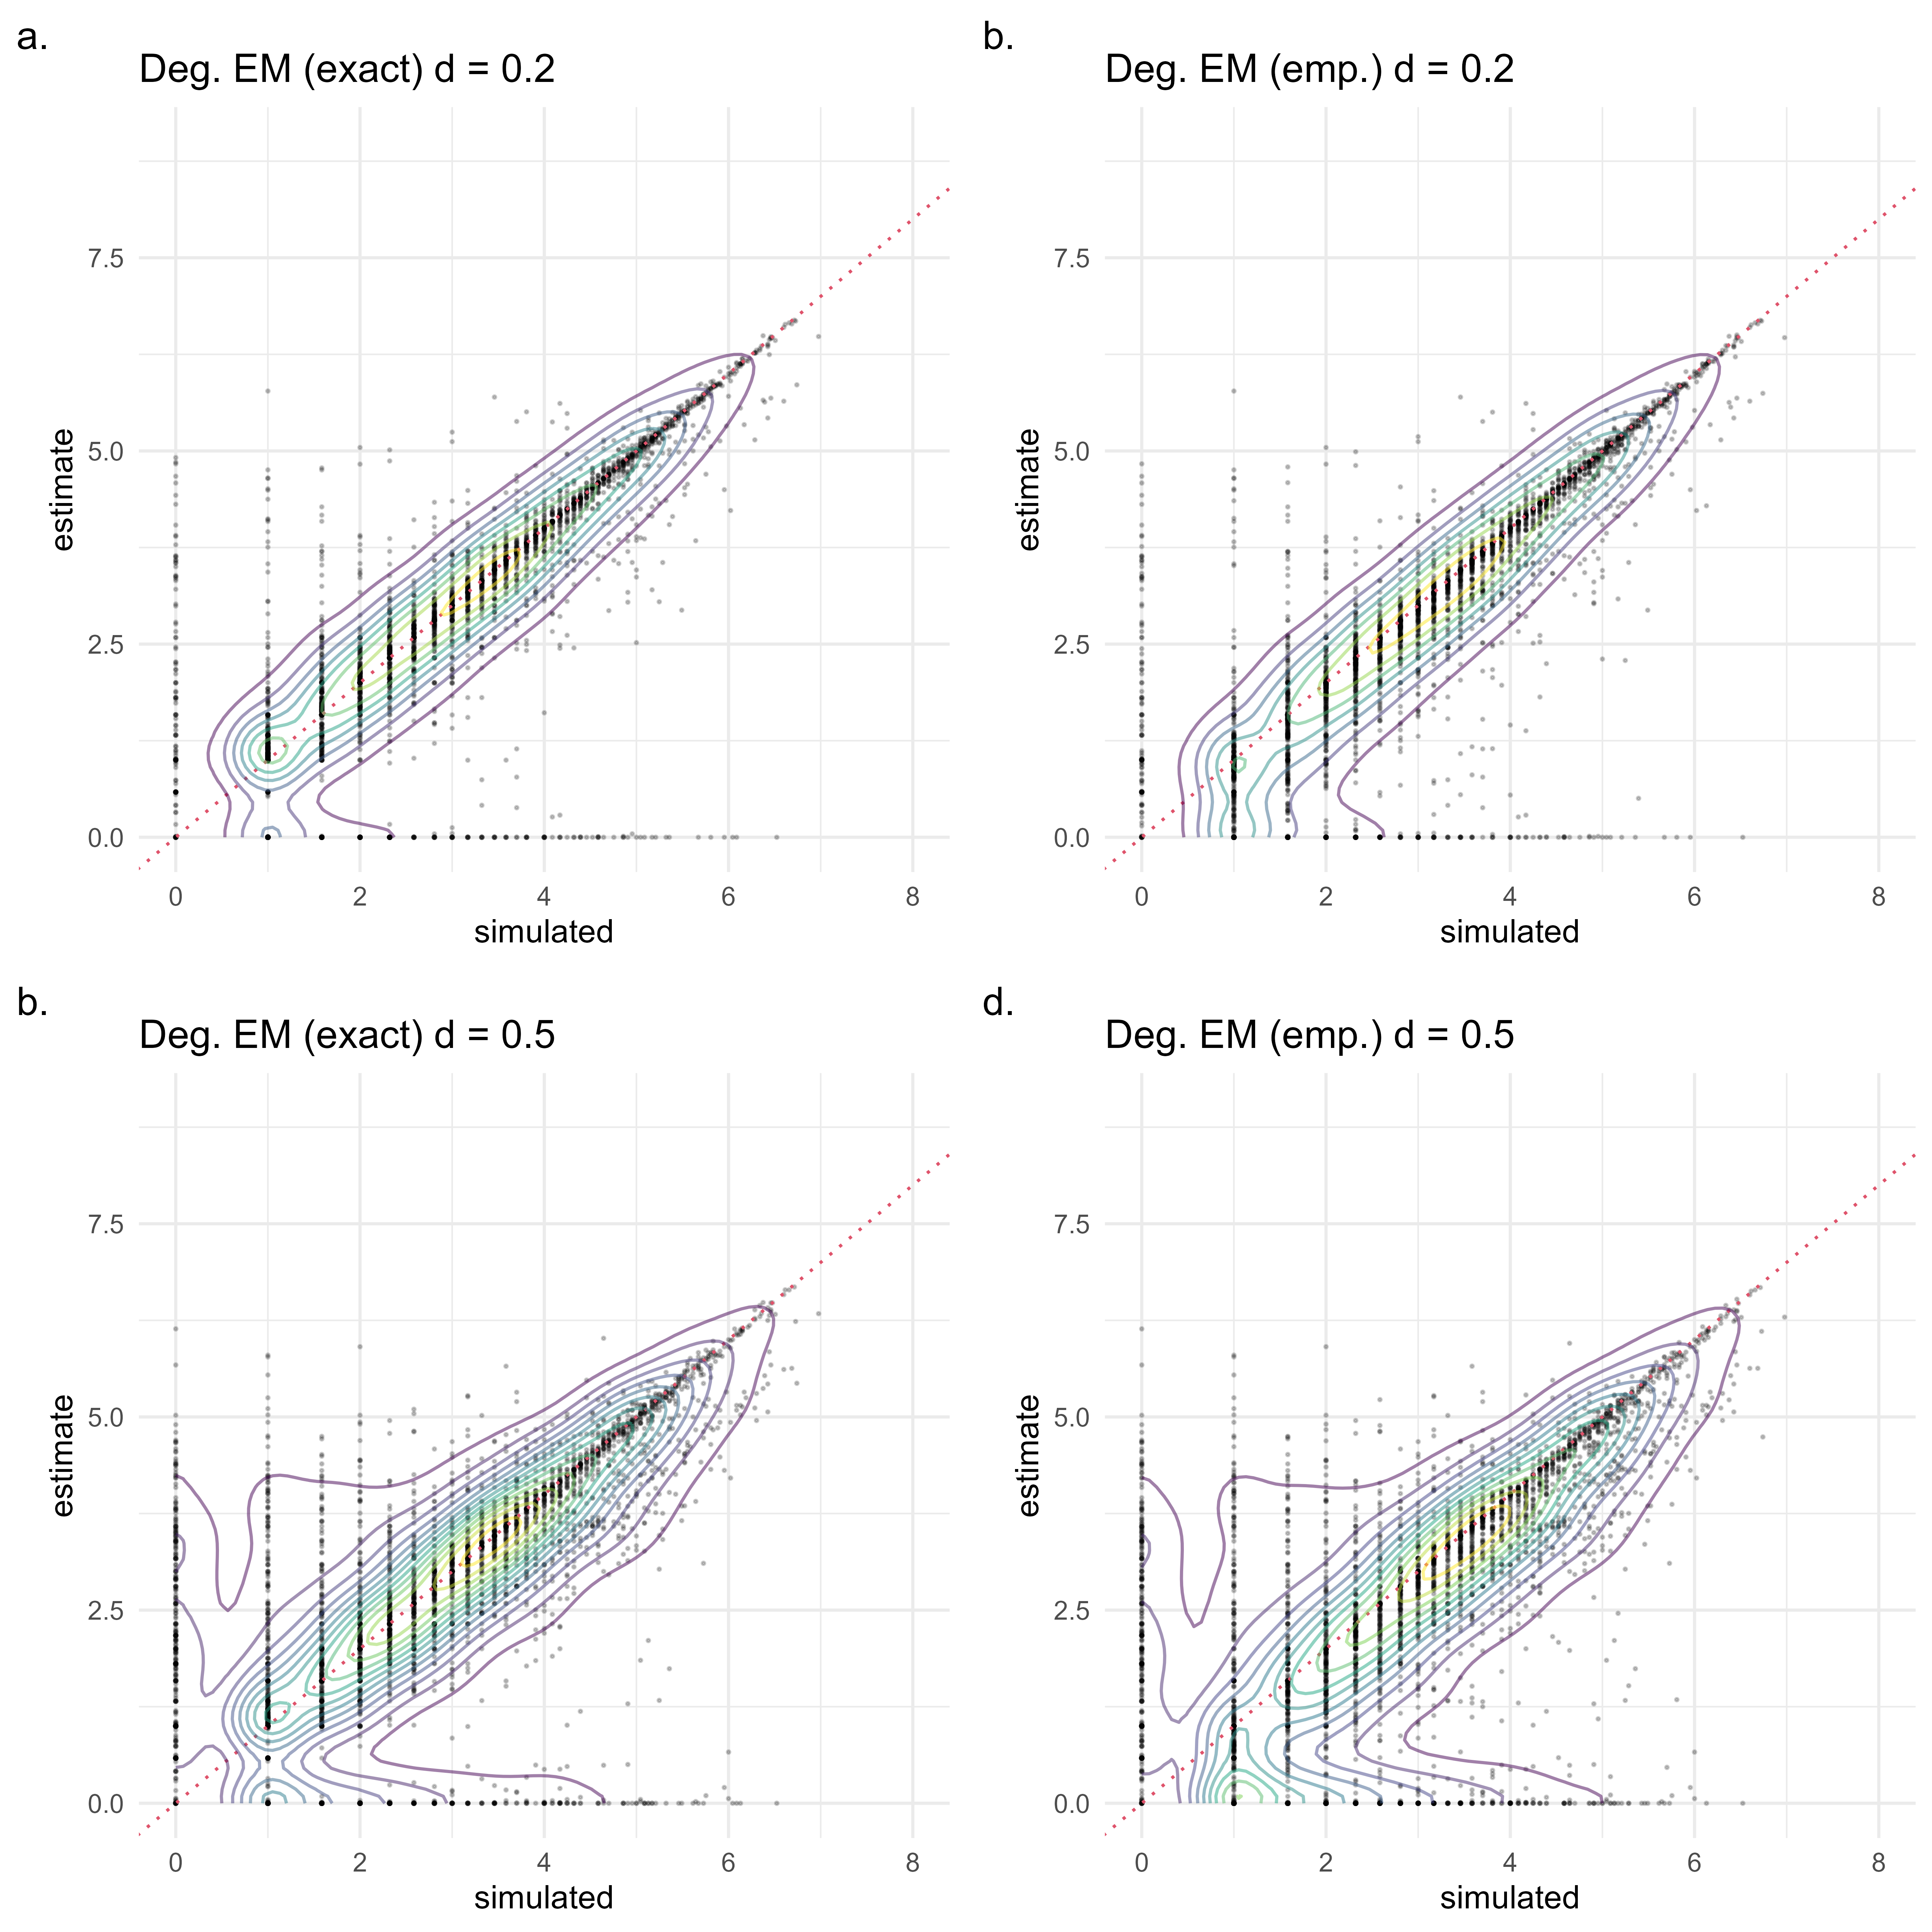
\includegraphics[width=\textwidth]{figures/sec-4-1-scatter-hard.png}
    \caption{Scatter}
    \label{fig:my_label}
\end{figure}


\begin{figure}[H]
    \centering
    \includegraphics[width=\textwidth]{figures/sec-4-1-scc-nrmse.png}
    \caption{SCC}
    \label{fig:my_label}
\end{figure}

\subsection{Comparisons with existing methods}

%[Empirical results for SCC and NRMSE on simulated datasets]{Spearman correlation coefficient (SCC) and normalized root-mean-squared error (NRMSE) on simulated datasets with different degradation rates $\mathbb{E}[d]=\{0.05,0.1,0.2,0.4,0.5\}$. \textbf{a.} SCC across all simulated isoforms. \textbf{b.} SCC across subset isoforms. \textbf{c.} NRMSE across all simulated isoforms. \textbf{d.} NRMSE across all subset isoforms.

%[Scatter plots on subset isoforms for simulated data]{Scatter plots on subset isoforms in a simulated dataset with $\mathbb{E}[d]=0.2$ across the methods. Counts are $\log_2$ transformed with the addition of 1 pseudocount. A kernel density (KDE) is fitted to show the density of points. No KDE is fitted for flair due to the abundance of zeroes. The diagonal is indicated by the dotted line.

%[Empirical results for degradation rate estimation on simulated datasets]{Comparison of the degradation rates estimated by bambu and our model on simulated datasets with different degradation rates $\mathbb{E}[d]=\{0.05,0.1,0.2,0.4,0.5\}$. The diagonal is indicated by the dotted line.

\section{Evaluations on real data}

Six H9 samples (600ng mRNA + 1\% spike-in of 6ng SIRV-4) sequenced with direct RNA-seq.

\subsection{Comparisons with existing methods}